\documentclass[a4paper,11pt]{article}
\usepackage[utf8]{inputenc}
\usepackage[italian]{babel}
\usepackage[maxbibnames=99,backend=bibtex]{biblatex}
\usepackage{hyperref}
\usepackage{listings}
\usepackage{color}
\usepackage{graphicx}

\addbibresource{ref.bib}
\graphicspath{ {images/} }

% define the title
\author{Luigi Leonardi}
%\pagestyle{headings}

\title{Tirocinio su Posit}
\date{}


\definecolor{mygreen}{rgb}{0,0.6,0}

\lstset{  
	numbers=left,
	numbersep=5pt,
	commentstyle=\color{mygreen},
	keywordstyle=\color{blue}\ttfamily,
	stringstyle=\color{red}\ttfamily  
}


%link cliccabili
\hypersetup{colorlinks=true, linktoc=all,  linkcolor=black,citecolor=black}

\begin{document}
	% generates the title
	\maketitle
	% insert the table of contents
	\tableofcontents
	
%	\cite{epfl1}
	

\newpage
	\section{Introduzione}
	\subsection{Posit}

	Il Posit è un formato di numero in virgola mobile ideato da John Gustafson, in alternativa allo standard IEEE 754. L'idea di base è fondamentalmente la stessa, anche nei Posit è presente un bit per il segno, dei bit per l'esponente e dei bit per la mantissa, le principali differenze consistono nella presenza di un "super esponente" o regime e nel non avere un numero di bit fissato per quest'ultimo e per la mantissa. \\
	\begin{figure}[h]
	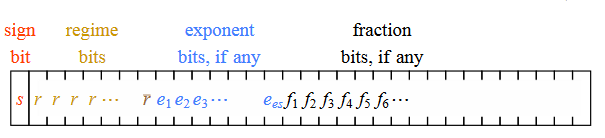
\includegraphics[scale=0.8]{posit}
	\centering
	\caption{"Formato Posit"}
	\end{figure}Il vantaggio nell'avere un super esponente, la cui lunghezza non è definita, permette di ottenere un range di numeri molto più flessibile, il suo contributo è pari a $2^{2^{es}}$ con es il numero di bit dell'esponente\footnote{L'esponente è l'unico campo ad avere una dimensione fissa}, permettendo quindi una riduzione del numero di bit assegnati a quest'ultimo campo oppure un incremento di range.\newline Questi bit di regime non sono altro che una sequenza di cifre binarie identiche, terminate dal complemento di esse. \newline Ad esempio: 0001 rappresenta -3, dove 3 è il numero degli 0 ed 1 è il terminatore.\footnote{Regimi che iniziano per 0 sono negativi, per 1 invece sono positivi. Lo 0 è rappresentato come 10}\cite{epfl1}
	
	\subsection{Note sui Test}
	Tutti i test svolti sui Posit sono stati effettuati sfruttando la libreria in C++ BFP\cite{libbfp} 
	implementando, dove necessario, le funzionalità mancanti.\newline I Posit scelti sono stati a 32/64 bit, con 0 bit di esponente\footnote{Ha senso non utilizzare bit di esponente, in quanto si sfrutta il super esponente}, dove non specificato diversamente.
	
%	\subsection{Cippi}
%	\ldots{} ora e' in distilleria.
\newpage
\section {Test}
\subsection{Accuratezza}

Questo test vuole dimostrare che a parità di bit utilizzati, 32 in questo caso, i Posit risultano essere più precisi nel rappresentare i risultati di prodotti, rispetto ad un Float in precisione singola.\\
In questo particolare caso sono stati impiegati Posit [32,3], ossia 32 bit totali, di cui 3 di esponente.
\subsubsection{Svolgimento}
Il test consiste nel creare 9 array, 6 per gli operandi e 3 per i risultati, di una dimensione compresa nell'ordine dei milioni: \begin{itemize}
	\item 3 di Posit [32,3]
	\item 3 di Float a 32 bit 
	\item 3 di Double a 64 bit come riferimento
\end{itemize} Il passo successivo consiste nel popolare gli array degli operandi, operazione che viene svolta partendo dai double sfruttando una funzione che genera dei numeri in modo pseudo-casuale, per poi provvedere a riempire gli altri semplicemente operando le necessarie conversioni.\\
Successivamente sono state eseguiti i vari prodotti i cui risultati sono stati collocati nel terzo array di ciascun tipo. Infine, per poter confrontare il tutto, i risultati sono stati riportarti in double e ne è stata fatta la differenza, in modulo, rispetto al riferimento.\\\\ Definisco: \begin{center}  $\Delta_i$(Posit) = $|PositRes_i - DoubleRes_i|$  \\ $\Delta_i$(Float)  = $|FloatRes_i - DoubleRes_i|$ \end{center} 
Dove FloatRes e PositRes sono il risultato del prodotto, fra float e posit rispettivamente, convertiti in double. \\Se $\Delta_i$(Posit) $<$ $\Delta_i$(Float) i posit sono più precisi dei float per questo indice.\\ Se $\Delta_i$(Posit) $>$ $\Delta_i$(Float) i float sono più precisi dei posit per questo indice.

\subsubsection{Conclusioni}
Dai risultati dei test svolti, i Posit si sono rivelati essere più precisi dei Float nel $\approx56$\% dei casi. Sono risultati pari merito nel $\approx16$\% dei casi.\\
I risultati risultano essere in linea con le aspettative, in quanto una maggiore precisione, a parità di dimensione, è imputabile ad un numero maggiore di bit disponibili per la mantissa, rispetto ai Float. 

\subsubsection{Codice}
\begin{lstlisting}[language=C++]
//Funzione per Numeri Random
double genererateNumber(){	// numeri fra -30 e 30
	double tmp = (double)rand()/(double)RAND_MAX;
	
	return (tmp*60) -30;
}


\end{lstlisting}


\section{Codice?}
\subsection{Test Sigmoide}
\begin{lstlisting}[language=C++]
	//Prova.cpp
	printf("Ciao");
	
	
\end{lstlisting}
	


\newpage

	\nocite{articolo1}
	
	\printbibliography[title=Bibliografia]

	

\end{document}